\documentclass{article}
\usepackage[utf8]{inputenc}
\usepackage{graphicx}
\graphicspath{ {images/} }
\usepackage{fullpage}
\linespread{1.5}

\title{Safe Execution of Untrusted x86 Machine Code Using Hardware-Assisted Virtualization}
\author{Yi-Fan Zhang}
\date{January 2017}

\newcommand{\PROJNAME}{\textit{hvexec}}

\begin{document}

\maketitle

\begin{abstract}
The ability to confine user-space software is critical for protecting users from
malicious or dubious application behavior.
With that in mind, we designed and implemented \PROJNAME{}, a virtualization layer that is interposed between applications and the kernel. Clients of \PROJNAME{} are given an API which they can use to monitor, filter or transform system calls from any application. To achieve this without requiring re-compiling or editing the application binary, we implemented \PROJNAME{} using an atypical application of hardware-assisted virtualization
where the restricted software executes in the context of a hardware virtual machine.
In this paper, we describe the benefits of using virtualization, the design and lessons learnt from our implementation and benchmarks to 
weight the benefits against the overhead.
\end{abstract}

\section{Introduction}
Local operating system security has traditionally focused on policing user interactions on multi-user systems \cite{DesignImplFreeBSD}.
However, in recent years, the pervasive use of personal computing along with the convenience of downloading
applications from the Internet has shifted the focus from restricting user privileges to limiting capabilites per application process
— sometimes referred to as sandboxing, application compartmentalization or process mitigation \cite{DesignImplFreeBSD}.
While conventional OS access controls based on notions such as users and groups have proven to be valuable,
they become awkward tools for applying security policy definitions on a per application basis \cite{DesignImplFreeBSD}.
Although numerous approaches to solve this particular problem have been proposed (see related works),
research into the best designs for applying sandboxing to software along with methods for decreasing overhead, remains active \cite{Ayer2012,VCall2010,DesignImplFreeBSD}.

In this paper, we propose \PROJNAME{}, an application sandbox designed to protect users from malicious or dubious application behavior.
To his end, we designed \PROJNAME{} against these principles:
\begin{itemize}
    \item \textbf{Resource Control:}
        Any access to system resources must be delegated through the sandbox.
    \item \textbf{Fidelity:}
        Applications must be loaded as native executables with no modifications to the binaries
        (no recompilation or binary translation) and behave equivalently as running outside the sandbox.
    \item \textbf{Flexibility:}
        Users should be given an API to program custom policies while the burden of enforcement falls upon the sandbox.
    \item \textbf{Performance:}
        Sandboxed applications should run as close as possible to unsandboxed speed
        and performance must not degrade significantly as more concurrent sandboxed processes are started.
    \item \textbf{Safety:}
        The sandbox must not weaken, circumvent or introduce new vulnerabilites into conventional OS access controls.
\end{itemize}
To help meet those requirements, our sandbox incorporates strategies from various related works.
At the foundation, we based \PROJNAME{} on an atypical application of hardware virtualization extensions (Intel VT-x) where
the sandboxed software (guest) executes in the context of a hardware virtual machine (HVM).
The hardware enforced nature of the virtual machine (VM) implicitly provides the advantage that the guest runs completely out-of-band with the host OS software.
By simulating a complete hardware environment within the VM, the guest has its own set of processor registers, physical memory and privilege modes.
More importantly, this requires the guest to cross a VM to host boundary before it can access any host resources
— similar to the hardware protection facilities provided for switching between user and kernel mode which is fundamental to implementing a reliable and secure operating system.
We exploit this property by dividing \PROJNAME{} into two parts: one runs as a user process on the host and another in kernel mode in the VM.
This assures that all guest system calls and accesses to privileged memory ranges can be trapped, and
by running \PROJNAME{} as an unprivileged user process on the host, we implicitly subject the
entire sandbox system to existing OS access control restrictions.
As part of the fedelity requirement, sandboxed applications must also not be able to detect the presence of the sandbox.
Otherwise, applications may choose to deny the user services in order to coerce permissions to be granted.

Aside from providing resiliance and isolation, \PROJNAME{} improves on prior work in terms of flexibility and performance.
In terms of flexibility, \PROJNAME{} exposes a user programmable API for defining security policies rather than a prescribed system wide security model commonly seen in previous approaches.
This returns control to the users while future proofing the system against the rapid changes in application development.
Furthermore, we mitigate the risk of introducing new system vulnerabilities by leveraging existing kernel support for virtualization hardware
such that no additional kernel modules need to be installed and no administrator privileges are needed to run \PROJNAME{}.
Although programs can execute natively within a VM, frequent context switching between VM and host can degrade performance.
We address this problem with a novel application of exitless notifications \cite{ELI2015} for VM and host communication that avoids
context switching entirely.

To validate our design, we provide an implementation of \PROJNAME{} built on OS X 10.11.4 — an operating system with
a rich set of user applications and kernel support for HVM.
For our evaluation, we weighed the benefits provided by \PROJNAME{} against the overhead using a suite of benchmarks on graphical and commandline applications as well as
microbenchmarks simulating worst case performance scenarios.
While the total virtualization overhead can be amortized over the total execution of the program \cite{Ayer2012, VCall2010}, the immediate affect on latency
sensitive applications has not been measured.
Similarily, the feasibility of scaling to hundreds of HVM sandboxed proccesses in is not known.
Thus, we also focused our investigation on aspects of scalability and context switching latency that were not previously examined.

In summary, we have proposed an application of hardware-assisted virtualization aimed at solving the problem of software confinement.
Our contributions include providing a user-programmable security system and a method of mitigating VM context switching latency.
Lastly, we believe the virtualization cost is well justified by the benefits attained, and we confirm our findings by benchmarks on \PROJNAME{} which we have also made open source.

The rest of the paper is organized as follows:
Section 2 compares \PROJNAME{} with related work.
Section 3 describes the design issues we faced and our solutions.
Section 4 presents benchmarks to evaluate \PROJNAME{}.
Section 5 suggests future direction and concludes the paper.

\section{Related Work}
In this section, we compare \PROJNAME{} with several representative works.
Our comparison does not imply that other approaches are not suitable for their original usage scenarios.
Instead, we intend to show that \PROJNAME{} improves on prior designs for addressing the requirements in the introduction section.

Directly modifying the kernel is the most direct approach and can achieve the best performance as well as offering excellent assurances.
Within the Linux community, SELinux (Security Enhanced Linux) has been in use since the late 2000s \cite{SELinux2006}.
SELinux adds finer granularity to existing access controls and allows the system's administrator be able to specify which users an read, write, append, unlink, move or execute a file and so on \cite{SELinux2006}.
Unlike existing access controls, SELinux can also enforce restrictions on network access and inter-process communication channels \cite{SELinux2006}. However, kernel extensions requires nontrivial code changes to kernel which has risk of introducing new vulnerabilities \cite{ptrace2002, ptrace2003} and requires recompiling the kernel and elevated permissions for installation which inconveniences users and administrators.
Solutions like SELinux typically prescribe a fixed (non-programmable) security model whereas we aim to provide general purpose programmability.
Other existing kernel features like ptrace are not suited for sandboxing due to argument race conditions \cite{ptrace2003}.
Shill Shell and Capsicum on FreeBSD provide programmable capability-based interface \cite{capsicum2010, shillshell2014}. However, the Shill Shell relies on FreeBSD's MAC framework which limits the granularity at which it can protect resources. Both do not support transformations on arguments and return values from system calls.

Alternatively, implementing a sandbox purely in userspace has been explored in prior works, most notably, Google's Native Client (NaCl) \cite{nacl2009, nacl2011}.
NaCl avoids the performance overhead of dynamic binary translation by statically verifying machine code at compile time \cite{nacl2009}.
To address the difficulty on architectures with variable length instructions and jump targets not aligned to instruction boundaries binaries, NaCl requires that no instructions or pseudo-instructions overlap a 32-byte boundary.
In short, in order to make this type of analysis feasible, NaCl imposes specific constraints on the pattern of machine instructions used \cite{nacl2009}.
Our approach allows arbitrary sequences of machine code to be executed without any static analysis binary translation.

The last category leverages the widespread deployment of virtualization capable hardware (HVM) to do sandboxing.
While full OS Virtualization provides the necessary isolation is not scalable because of the large overhead of running an entire guest operating system.
This motivates the need for implementing a more specific light-weight solution.
The most similar existing works that we were able to find are Ether, VCall, KVM sandbox and Microsoft Application Guard \cite{Ether2008, Ayer2012, VCall2010, msft2016}.
Each is either implemented using KVM on Linux or Hyper-v on Windows.
To the best of our knowledge, there is currently no implementation for macOS.

\section{Design and Implementation}
The primary responsibility of \PROJNAME{} is to isolate any side effects that an arbitrary untrusted sequence of x86 machine code may have on the underlying system.
One can simply think of \PROJNAME{} as two components: the untrusted code which executes inside a VM and the management program running on the host as a normal user process.
As described in the introduction, the VM serves as a native execution environment that is isolated from the host at the hardware level.
To access any host side resource, the untrusted code in the VM must trigger a VMEXIT condition which turns the execution over to the management program on the host.
By interposing on these VMEXIT events, we are able to control what resources the untrusted code can see and use as shown in Figure 1.

\begin{figure}[ht]
    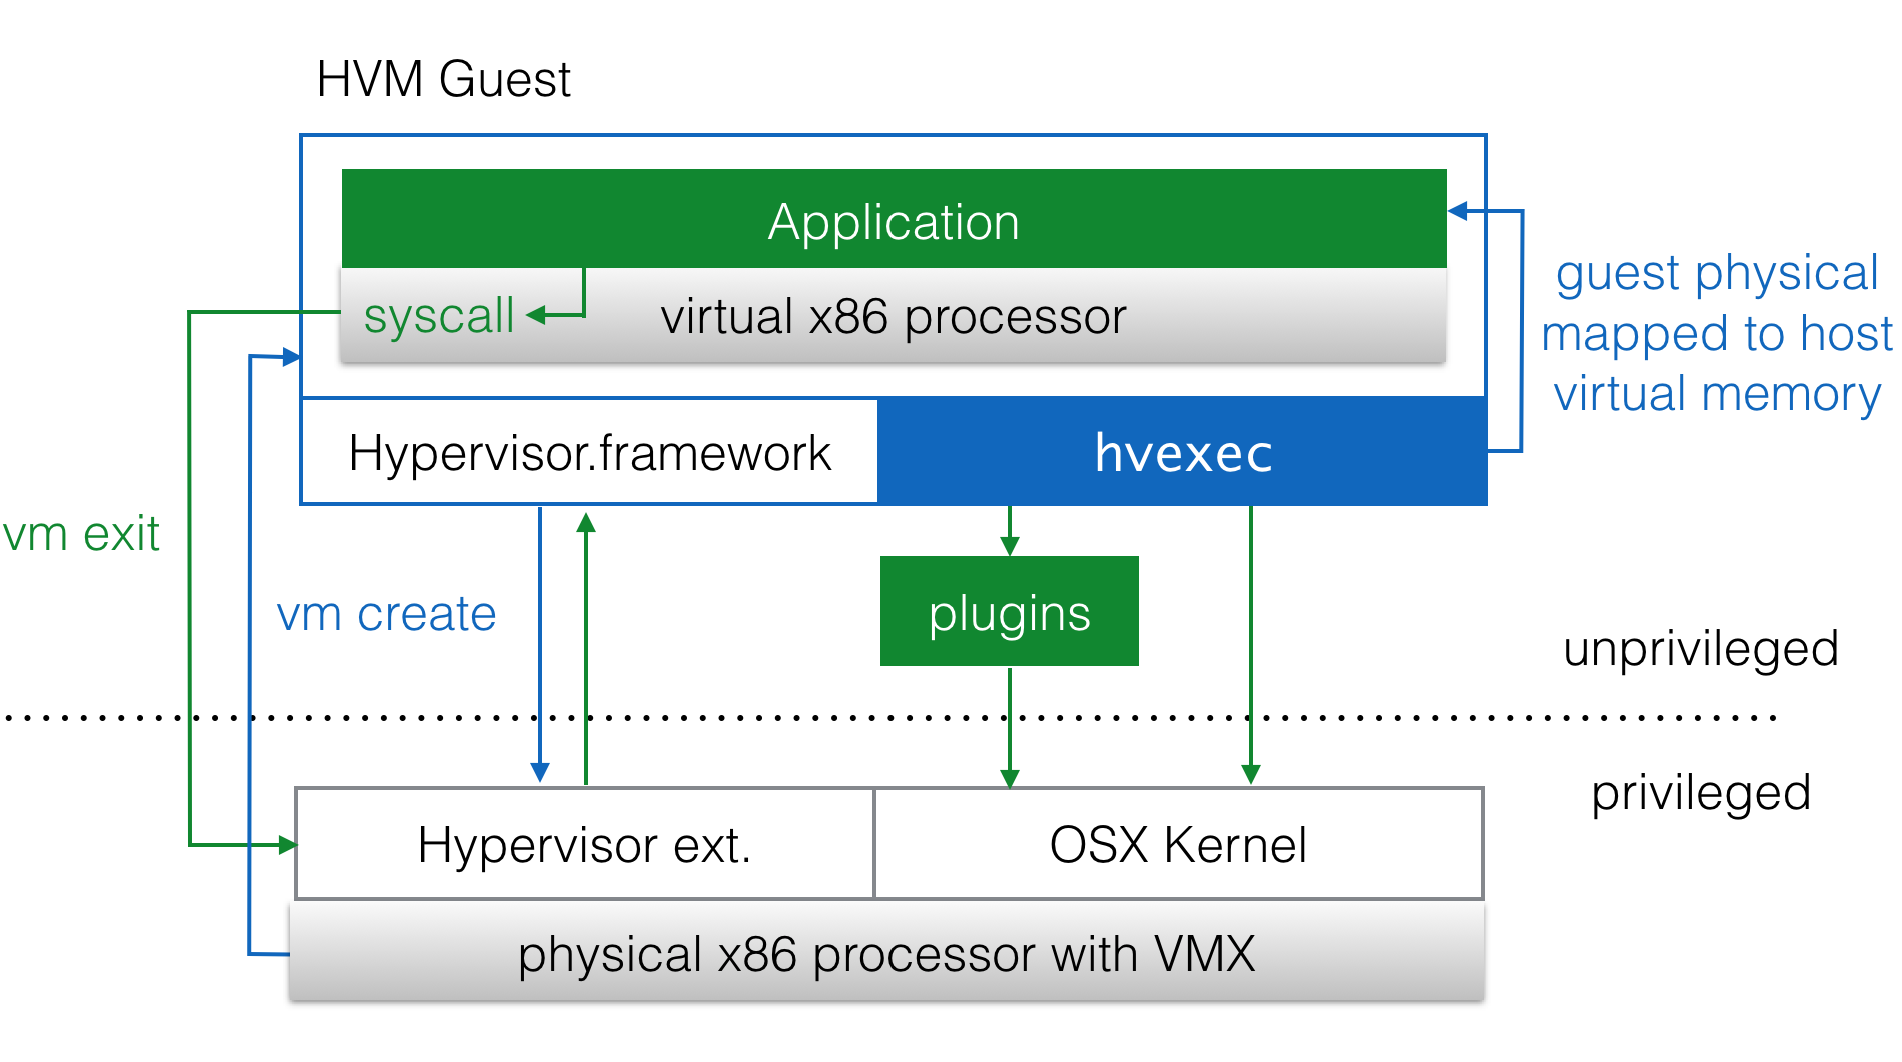
\includegraphics[width=16cm]{hvm}
    \caption{Diagram showing sandbox creation and system call interposition}
    \centering
\end{figure}

We chose to build the prototype on macOS, a popular operating system among consumers and application writers in this era.
MacOS has kernel support exposing the underlying x86 VT-x extensions through a system called \texttt{Hypervisor.framework} (analogous to KVM on Linux).
The rest of this section will describe how \PROJNAME{} manages memory, interposes on system resource access and exposes a programmable API. It is organized as follows: Section 3.1 initialization Section 3.2 address translation. Section 3.3 syscall handling. Section 3.4 explains the plugin system. Section 3.5 addresses current limitations.

\subsection{Initialization}
We designed \PROJNAME{} to be used as a command-line application.
Upon start-up, \PROJNAME{} needs to create a new VM using the API exposed by \texttt{Hypervisor.framework}.
\texttt{Hypervisor.framework} enforces a one-to-one mapping between VM and host process; however, each VM may be configured with one or more virtual CPUs (VCPU). Each VCPU may be mapped to a host thread.
While \texttt{Hypervisor.framework} handles some of the setup, the client is expected to do most of the configuration.
VM creation involves configuring the register state of VCPUs, the conditions for VMEXITs and the physical memory allocation for the VM.
Most of this configuration is done by setting specific fields in an in memory structure called the Virtual Machine Control Structure (VMCS) \cite{intelmanual}.
The exact definition of each field can be referenced in Intel's official systems programming manual \cite{intelmanual}.

The VM is capable of supporting 16, 32 and 64 bit execution modes.
The 16 bit mode (real mode) is mostly used for legacy applications and firmware and most applications on macOS are compiled for 64 bit execution (IA-32e, also known as long mode).
Thus, we only aim to support x86\_64 machine code; however, we made \PROJNAME{} boot the VM in 32 bit mode, in case we want to add 32 bit support in the future, then transition to 64 bit.
For x86, 64-bit execution requires virtual memory to be enabled and it is \PROJNAME{}'s responsibility to setup the initial global descriptor tables and segment selector registers.
Lines 33 to 41 of \texttt{boot.asm} describe the initial memory layout.
To help determine the correct configuration values, we referenced an open source hypervisor called Xhyve and based our configuration on Xhyve's during the boot process.

\subsection{Address Translation}
Code in the VM (guest) executes in a separate address space than the host process.
The address spaces from guest to host are as follows: guest virtual address (GVA), guest physical address (GPA), host virtual address (HVA) and host physical address (HPA).
The guest is allowed to manage its own page tables, but \PROJNAME{} initializes the guest to use 4 Kbyte size pages.
Translation from GVA to GPA is performed by the MMU in the VM.
The mapping between GPA and HVA is tracked by means of a list of \texttt{struct mem\_region} nodes defined in \texttt{vm\_mem.c}. The function \texttt{gpa\_to\_hva()} in the same file implements the logic to traverse the list and look-up the address mappings. 
HVA to HPA translation is handled entirely by macOS.

It's important to point out that the address translation functions in \texttt{vm\_mem.c} are only called during VM initialization or after a VMEXIT has been triggered.
GPA to HPA translation is normally handled by the hardware MMU through x86 extended page tables (EPT) managed by \texttt{Hypervisor.framework}.
With EPT, two page tables are traversed on a guest TLB miss. The first is the guest's page table and the second is the EPT configured on the host by \texttt{Hypervisor.framework}.
This doubles the cost of a guest TLB miss.
To mitigate this cost, Intel added an Address Space Identifier (ASID) to
track which entry in the TLB belongs to which VM. This way, a context switch between VMs won't necessarily trigger a TLB flush.

\subsection{VMEXIT Handling}
Once initialization is complete, the \texttt{vcpu\_run()} function in \texttt{vcpu.c} is called.
Within this function, the program enters a run loop which performs the following logic on each iteration. 
First, \texttt{hv\_vcpu\_run()} is called and this transfers execution to a VCPU.
This is a blocking call and will only return when a VMEXIT condition is triggered.
This list describes the VMEXIT conditions handled by \PROJNAME{}.

\begin{itemize}
    \item \texttt{VMX\_REASON\_IRQ:}
        The time slice or quantum for the VM is up.
    \item \texttt{VMX\_REASON\_EXC\_NMI:}
        A non-maskable interrupt (NMI) was triggered. This most likely indicates an error condition since \PROJNAME{} does not explicitly use NMIs.
    \item \texttt{VMX\_REASON\_VMCALL:}
        The code in the VM executed the \texttt{vmcall} instruction. This instruction is used to explicitly trigger a VMEXIT. Currently it is used for debugging.
    \item \texttt{VMX\_REASON\_HLT:}
        The \texttt{hlt} instruction was executed and now the VM should terminate.
    \item \texttt{VMX\_REASON\_EPT\_VIOLATION:}
        Triggered when the VM references a memory location that has not been paged in. The page fault will be handled by macOS and \texttt{Hypervisor.framework}; however, if we wanted to implement MMIO, this is where it should be done.
    \item \texttt{VMX\_REASON\_RDMSR,VMX\_REASON\_WRMSR:}
        This is for handling reads and writes to model specific registers (MSR). Since we boot the VM in 32 bit mode, transitioning to 64 bit requires setting MSR values.
    \item \texttt{VMX\_REASON\_MOV\_CR:}
        Paging must be enabled in order to use 64 bit mode. To turn on paging the VM has to assert bit 31 in \texttt{cr0} (control register 0).
    \item \texttt{Default:}
        The \texttt{syscall} instruction normally does not trigger a VMEXIT. To force a VMEXIT we register an invalid syscall handler and trigger a triple fault. 
        Since the \texttt{syscall} instruction stores the next instruction address in the \texttt{rcx} register before jumping to the syscall handler, we can read the instruction at the address of \texttt{rcx} minus 2 bytes (size of the \texttt{syscall} insturction) to determine if the triple fault was caused by a \texttt{syscall}. If not, then this is an error condition. Otherwise, we handle the \texttt{syscall}.
\end{itemize}

In any non-error case, we also increment the value of \texttt{rip} (instruction pointer) to the next instruction. The run loop terminates when an unhandled error occurs or when the VM executes a \texttt{hlt}. 
 
\subsection{Plugin System}
When \PROJNAME{} is invoked on the command-line, the path to a plugin can be passed in as an optional argument.
The purpose of plugins is to allow users to implement their own programmable security policies.
If this argument is not supplied, \PROJNAME{} simply functions in pass-through mode and all system calls are forwarded to the host unmodified.

Plugins are macOS dynamic libraries (\texttt{*.dylib}) that conform the the interface defined in \texttt{hvexec\_plugin.h}.
The plugin writer is only required to implement the \texttt{plugin\_init()} function.
A \texttt{struct plugin\_ops} object is initalized by \PROJNAME{} and passed as an argument to \texttt{plugin\_init()} as a way for the plugin to hook into \PROJNAME{} events.
Function pointers can be optionally assigned to \texttt{plugin\_ops} to override default system call behavior.

\subsection{Limitations}
While some applications ship as single statically linked executable, most applications link against dynamic libraries.
It is the responsibility of the loader to map the dynamic libraries into the process address space and fill out the
symbol relocation tables and properly setup position independent code.
However, the dynamic loader that ships with macOS (\texttt{dyld}) is not compatible with \PROJNAME{} because it depends on concurrency support (\texttt{pthread} and \texttt{OSSpinLock}).
Currently, our implementation is limited to running single threaded applications.
We do not support system calls to OS level threading or fork() style multiprocessing and \PROJNAME{} only uses a single VCPU.
Although \PROJNAME{} only supports statically linked binaries, this does not preclude users from implementing their own dynamic loader and running that in the VM along with their application.


\section{Evaluation}
The only question remaining is the performance overhead of our approach which will be
addressed in the evaluation section.
Results for benchmarks.
\subsection{Compute Performance}
\subsection{Context Switching Overhead}
\subsection{Scalability}
Performance degradation when scaling to hundreds of processes.

\section{Conclusions}
Here we have documented \PROJNAME{}, a sandbox for safely executing untrusted x86 machine code.
We have shown how \PROJNAME{} can be used to guard against undesirable side effects on underlying system resources and evaluated the performance cost.
We hope to have convinced the reader that hardware-assisted virtualization has the potential for achieving a higher level of protection and control for users compared to previous technologies. However, \PROJNAME{} is simply a starting point. It is easy to imagine many other applications using this type of technology:

\begin{itemize}
    \item
        ABI compatibility layer reducing burden on the OS for maintaining binary compatible interfaces.
    \item
        Portable binaries across different operating systems and foreign system call emulation.
    \item
        Live snapshotting and migration for applications.
    \item
        Tools for debugging and tracing.
\end{itemize}

\begin{thebibliography}{99}

\bibitem{DesignImplFreeBSD}
M. K. McKusick, G. V. Neville-Neil and R. N. M. Watson.
\emph{The Design and Implementation of the FreeBSD Operating System}.
Addison-Wesley Professional,
2nd edition,
2014.
ISBN-13: 978-0321968975.

\bibitem{Ostia2004}
T. Garfinkel, B. Pfaff and M. Rosenblum.
Ostia: A Delegating Architecture for Secure System Call Interposition.
\emph{NDSS, The Internet Society}, 2004.

\bibitem{VCall2010}
B. Li, J. Li, T. Wo, C. Hu and L. Zhong.
A VMM-based system call interposition framework for program monitoring.
In \emph{Parallel and Distributed Systems (ICPADS), 2010 IEEE 16th International Conference on}, 2010.

\bibitem{Ayer2012}
A. Ayer.
KVMSandbox: Application-Level Sandboxing with x86 Hardware Virtualization and KVM.
Master's Thesis, Brown University, 2012.

\bibitem{ELI2015}
N. Amit, A. Gordon, N. Har'El, M. Ben-Yehuda, A. Landau, A. Schuster and D. Tsafrir.
Bare-metal performance for virtual machines with exitless interrupts.
\emph{Communications of the ACM, 59}(1). 2015.

\bibitem{Ether2008}
A. Dinaburg, P. Royal, M. Sharif and W. Lee.
Ether: malware analysis via hardware virtualization extensions.
In \emph{Proceedings of the 15th ACM conference on Computer and communications security}.
ACM, 2008.

\bibitem{SELinux2006}
F. Mayer, D. Caplan, and K. MacMillan.
SELinux by example: using security enhanced Linux.
\emph{Pearson Education}, 2006.

\bibitem{ptrace2002}
W. Purczynski and A. P. Moore.
Vulnerability note VU\#176888, Linux kernel contains race condition via ptrace/procfs/execve.
CERT.org, 2002.

\bibitem{ptrace2003}
A. Cox.
CAN-2003-0127, Linux kernel ptrace() flaw lets local users gain root privileges.
cve.mitre.org, 2003.

\bibitem{shillshell2014}
S. Moore, C. Dimoulas, D. King and S. Chong.
SHILL: A secure shell scripting language.
In \emph{11th USENIX Symposium on Operating Systems Design and Implementation}. 2014.

\bibitem{capsicum2010}
R. N. Watson, J. Anderson, B. Laurie, K. Kennaway.
Capsicum: Practical Capabilities for UNIX.
In \emph{USENIX Security Symposium (Vol. 46)}, 2010.

\bibitem{nacl2009}
B. Yee, D. Sehr, G. Dardyk, J. B. Chen, R. Muth, T. Ormandy, and N. Fullagar.
Native client: A sandbox for portable, untrusted x86 native code.
In \emph{2009 30th IEEE Symposium on Security and Privacy}. 2009.

\bibitem{nacl2011}
J. Ansel, P. Marchenko, U. Erlingsson, E. Taylor, B. Chen, D. L. Schuff and B. Yee.
Language-independent sandboxing of just-in-time compilation and self-modifying code.
In \emph{ACM SIGPLAN Notices (Vol. 46)}. 2011.

\bibitem{msft2016}
Introducing Windows Defender Application Guard for Microsoft Edge.
https://blogs.windows.com/msedgedev/2016/09/27/application-guard-microsoft-edge/\#t7eWrQizF5YCMBiU.97

\bibitem{intelmanual}
Intel® 64 and IA-32 Architectures Software Developer’s Manual.
Volume 3 (3A, 3B, 3C \& 3D): System Programming Guide.

\end{thebibliography}

\end{document}

